\clearpage
\section{Ableitungstabelle}

\begin{center}
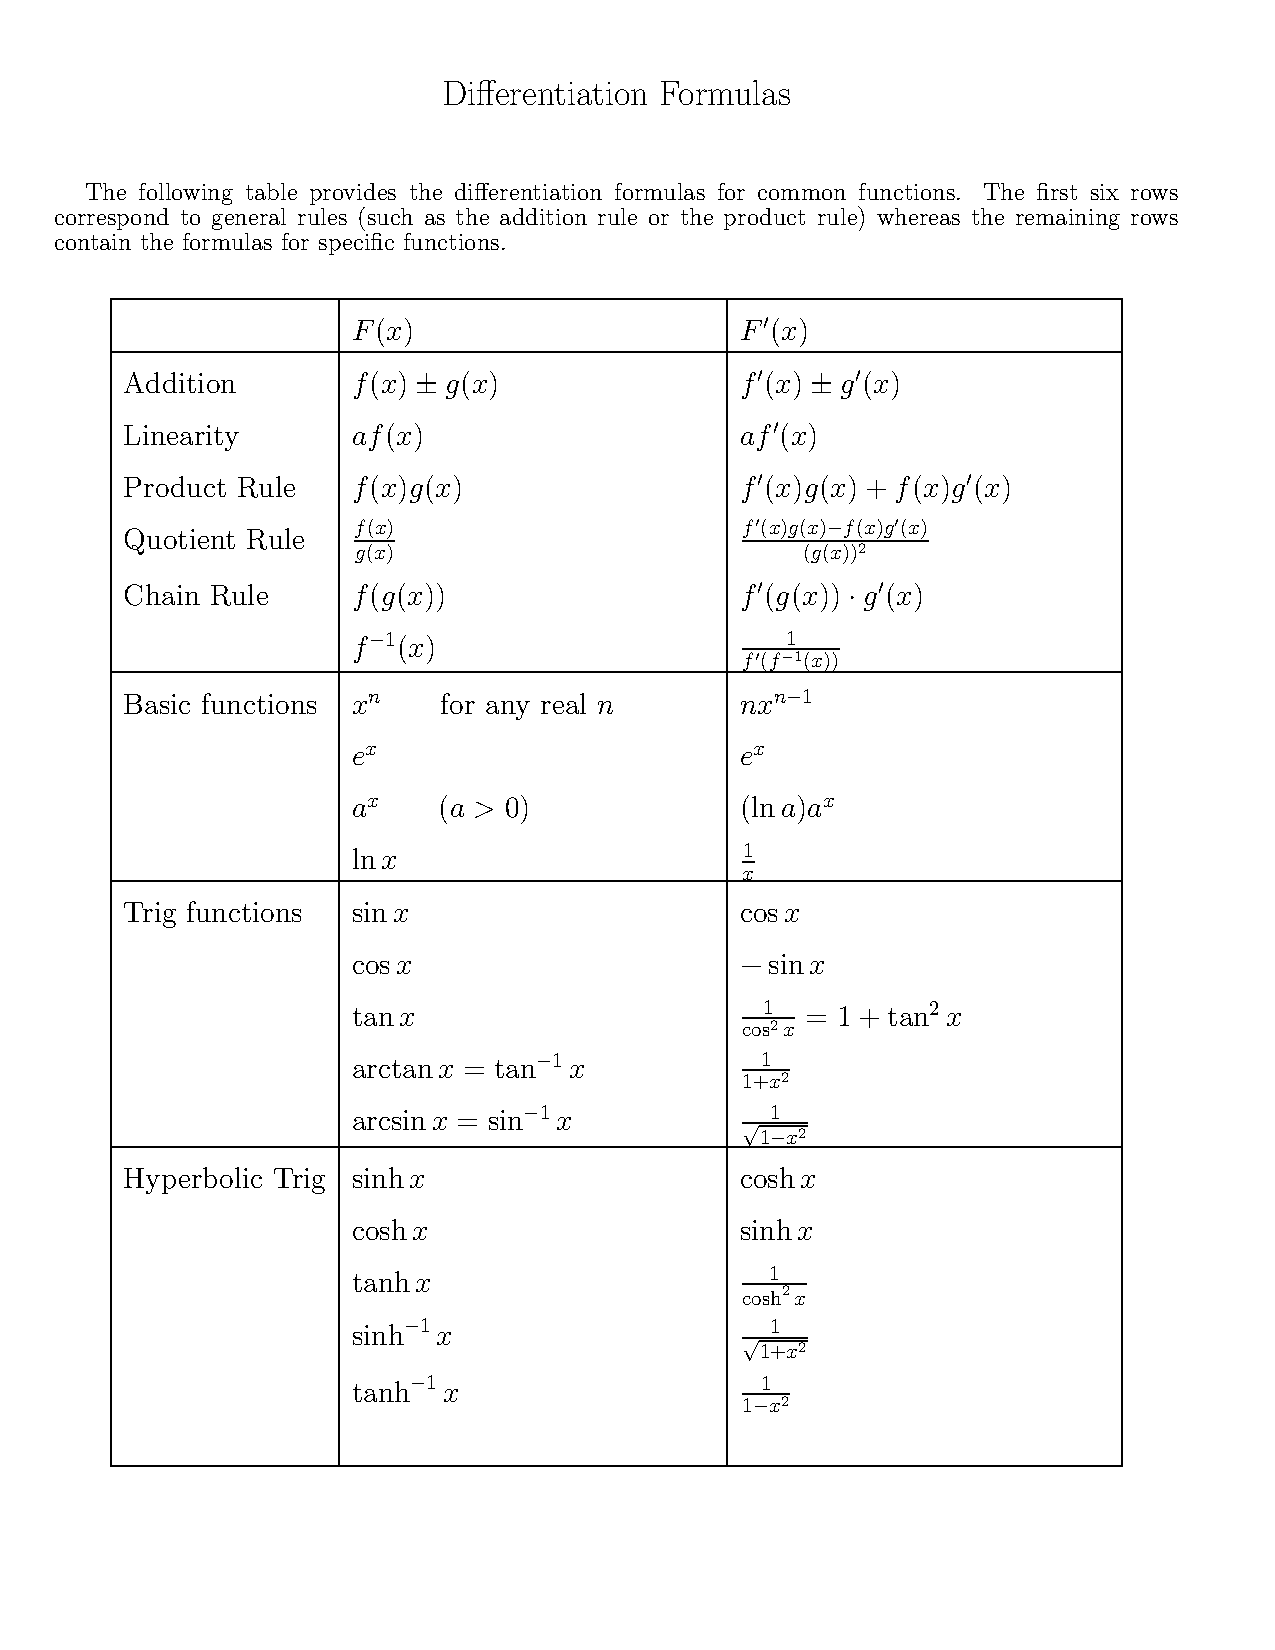
\includegraphics[page=1,width=14cm,trim=1.75cm 3.0cm 2.5cm 5.0cm,clip]{./files/calcrulz.pdf}
%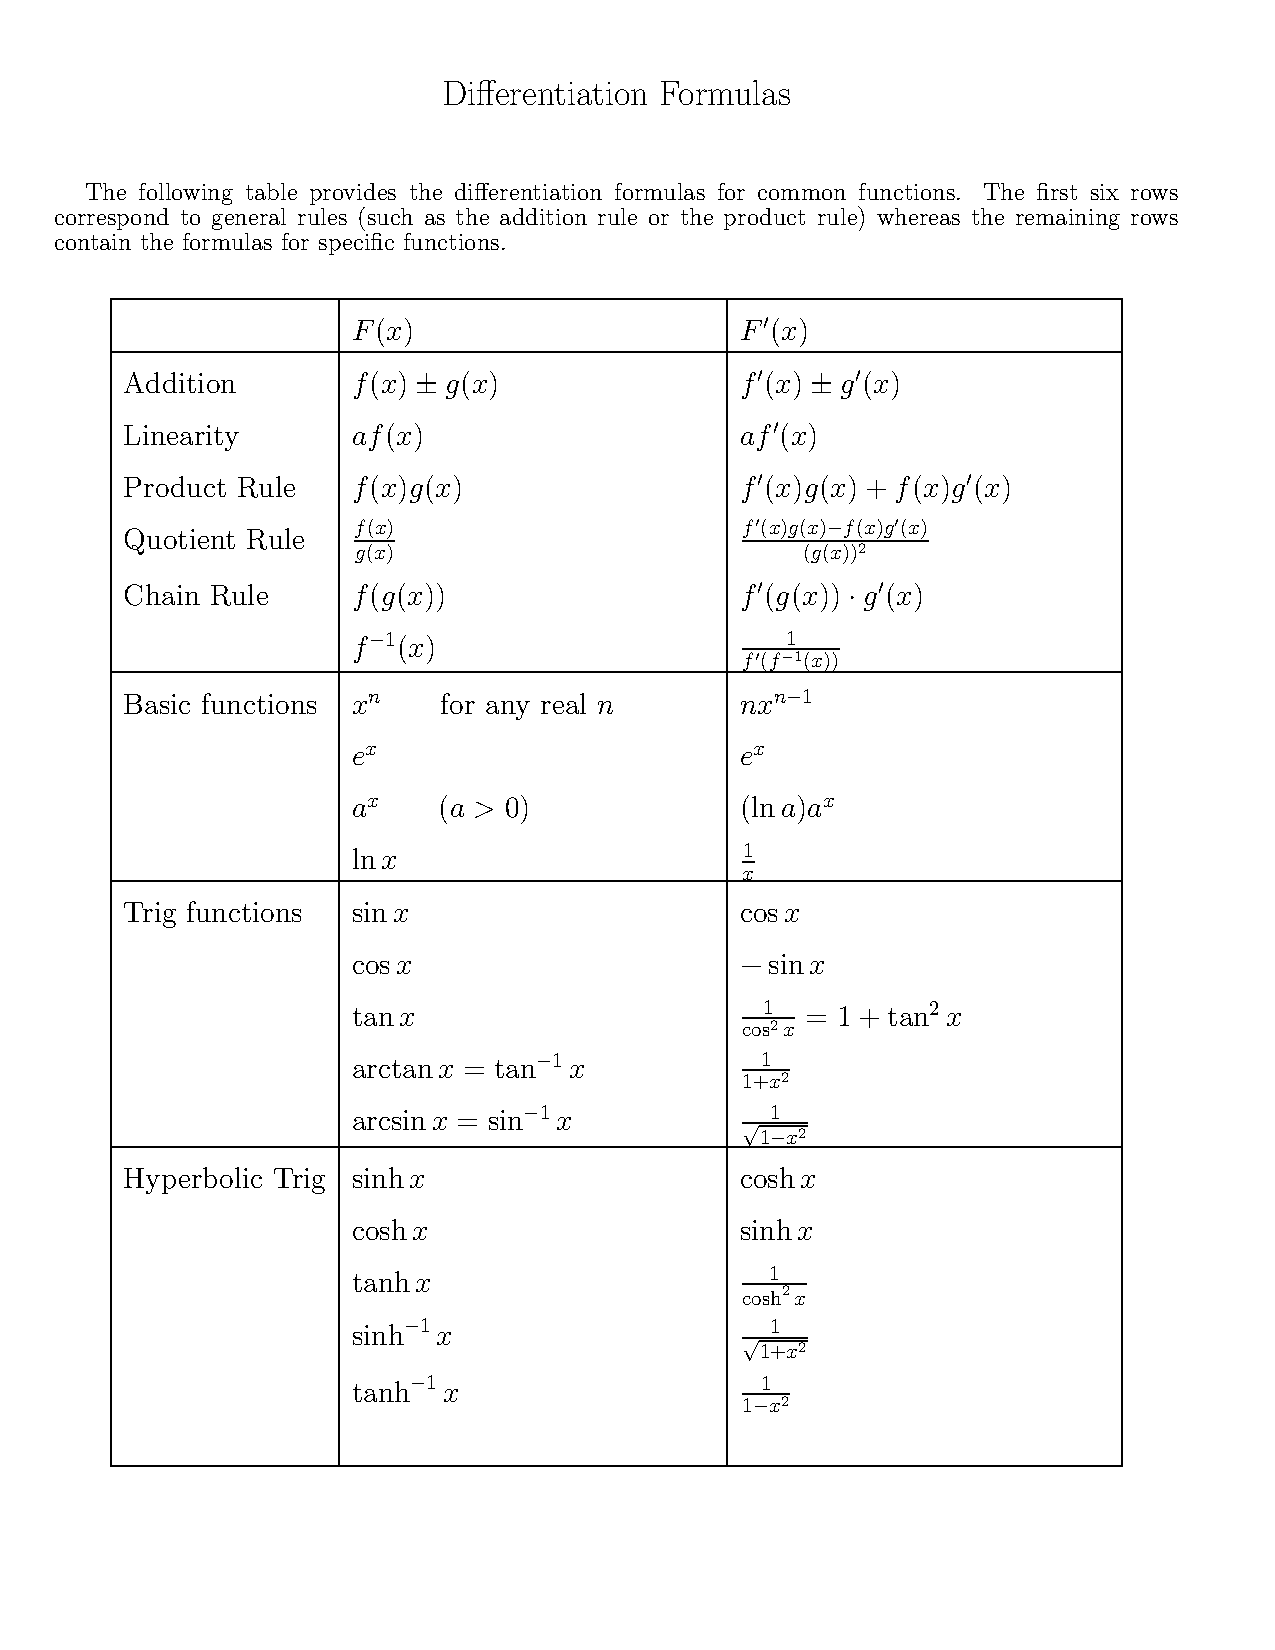
\includegraphics[page=1,width=14cm,clip]{./files/calcrulz.pdf}
\end{center}
\hfill
\section{Übersicht der Polynome}
\begin{tabular}{l|ll}
Name & Formel & Beispiel\\
\hline
Newton    & $\pi_n(x) =\prod_{i=1}^n(x-x_{i-1})$  & $\pi_2=(x-x_0)(x-x_1)$\\
Monomials & $x^n$                       & $x^2$\\
Bernstein & $B_{i,n}(x)=\binom{n}{i}(1-x)^{n-i} x^i$   & $B_{1,2}=2x(1-x)$\\
Chebyshev & $T_n(x)=\cos(n \arccos(x))$ & $T_2=2x^2-1$ 

\end{tabular}
\newpage

\section{Integrationstabelle}

\begin{center}
\includegraphics[page=2,width=18cm,trim=1.25cm 3cm 4.5cm 4cm,clip]{./files/calcrulz.pdf}
%\includegraphics[page=2,width=18cm,clip]{./files/calcrulz.pdf}
\end{center}
